%%%%%%%%%%%%%%%%%%%%%%%%%%%%%%%%%%%%%%%%%
% a0poster Landscape Poster
% LaTeX Template
% Version 1.0 (22/06/13)
%
% The a0poster class was created by:
% Gerlinde Kettl and Matthias Weiser (tex@kettl.de)
%
% This template has been downloaded from:
% http://www.LaTeXTemplates.com
%
% License:
% CC BY-NC-SA 3.0 (http://creativecommons.org/licenses/by-nc-sa/3.0/)
%
%%%%%%%%%%%%%%%%%%%%%%%%%%%%%%%%%%%%%%%%%

%----------------------------------------------------------------------------------------
%	PACKAGES AND OTHER DOCUMENT CONFIGURATIONS
%----------------------------------------------------------------------------------------

\documentclass[12pt,haverford,landscape]{haverposter}

\usepackage{multicol} % This is so we can have multiple columns of text side-by-side
\columnsep=100pt % This is the amount of white space between the columns in the poster
\columnseprule=3pt % This is the thickness of the black line between the columns in the poster

\usepackage[svgnames]{xcolor} % Specify colors by their 'svgnames', for a full list of all colors available see here: http://www.latextemplates.com/svgnames-colors

%\usepackage{times} % Use the times font
%\usepackage{palatino} % Uncomment to use the Palatino font

\usepackage{graphicx} % Required for including images
\graphicspath{{figures/}} % Location of the graphics files
\usepackage{booktabs} % Top and bottom rules for table
\usepackage[font=small,labelfont=bf]{caption} % Required for specifying captions to tables and figures
\usepackage{amsfonts, amsmath, amsthm, amssymb} % For math fonts, symbols and environments
\usepackage{wrapfig} % Allows wrapping text around tables and figures
\usepackage{listings}


%include these lines if you want to use the LaTeX "theorem" environments
\newtheorem{theorem}{Theorem}[section]
\newtheorem{definition}[theorem]{Definition}
\newtheorem{lemma}[theorem]{Lemma}
\newtheorem{corollary}[theorem]{Corollary}

\begin{document}

%----------------------------------------------------------------------------------------
%	POSTER HEADER
%----------------------------------------------------------------------------------------

% The header is divided into three boxes:
% The first is 55% wide and houses the title, subtitle, names and university/organization
% The second is 25% wide and houses contact information
% The third is 19% wide and houses a logo for your university/organization or a photo of you
% The widths of these boxes can be easily edited to accommodate your content as you see fit

\begin{minipage}[b]{0.55\linewidth}
\veryHuge \color{NavyBlue} \textbf{The Penney Ante Problem} \color{Black}\\ % Title
\Huge\textit{Analysis using Markov Chains, \\ Martingales, and Combinatoric Techniques}\\[1cm] % Subtitle
\huge \textbf{Saleh Hindi}\\ % Author(s)
\huge Haverford College, Department of Mathematics\\ % University/organization
\end{minipage}
%
\begin{minipage}[b]{0.25\linewidth}
\color{DarkSlateGray}\Large \textbf{Contact Information:}\\
Department of Mathematics\\ % Address
Haverford College\\
370 Lancaster Ave, Haverford PA\\\\
Email: \texttt{shindi@haverford.edu}\\ % Email address
\end{minipage}
%
\begin{minipage}[b]{0.19\linewidth}
\raisebox{2cm}{

\includegraphics[width=15cm]{Haverford-logo.jpg} }% Logo or a photo of you, adjust its dimensions here
\end{minipage}

\vspace{1cm} % A bit of extra whitespace between the header and poster content

%----------------------------------------------------------------------------------------

\begin{multicols}{4} % This is how many columns your poster will be broken into, a poster with many figures may benefit from less columns whereas a text-heavy poster benefits from more

%----------------------------------------------------------------------------------------
%	ABSTRACT
%----------------------------------------------------------------------------------------

  \renewcommand{\abstractname}{\LARGE \textbf{Abstract}}
\color{Black} % Navy color for the abstract
\begin{abstract}
  \vspace{.25in}

\Large
Imagine a two player game where
each player is assigned a sequence, for example THTH and HTHH, and a coin is flipped until either player sees their sequence.
The first player to see their sequence appear wins.
Given two sequences, which sequence is expected to come first in the
sequence of coin flips? What is the probability of a certain player winning? Although these two
questions sound similar, the result is that in our example,
the expected number of turns for sequence A to appear is 20 and for B it is 18. Meanwhile, the probability
of A winning is 9/14 while the probability of B winning is 5/14. Additionally the game has the property
that for any sequence A chooses, B can always find a sequence that has a higher probability of winning.
These counterintuitive results are the core of the Penney Ante problem, discovered by Walter Penney
\cite{gardner}. My thesis will study this problem through three approaches based in Markov chains, martingales,
and a combinatoric approach.
\end{abstract}

%----------------------------------------------------------------------------------------
%	The Game
%----------------------------------------------------------------------------------------

\color{Black} % SaddleBrown color for the introduction

\section{\LARGE The Game}

\Large Let $(S_t)$ for $t \geq 1$ be a stochastic sequence of letters chosen uniformly and
randomly from a $q$-letter alphabet. Let $A=a_1a_2a_3...$ and $B=b_1b_2b_3...$ be sequences
of $n$ letters chosen from the $q$-letter alphabet. We say
sequence $A$ or $B$ wins if it is the first sequence to appear within $(S_t)$. Let $\tau_A$ and $\tau_B$ be
the number of turns for $A$ or $B$ to appear. Note that $\tau$ is not a random variable. We denote
the probability of $A$ winning as $P(\tau_A < \tau_B)$ and we denote the expected time for sequence
$A$ and $B$ to appear as $E(\tau_A)$ and $E(\tau_B)$.

%----------------------------------------------------------------------------------------
%	Markov Chains
%----------------------------------------------------------------------------------------

\color{Black} % DarkSlateGray color for the rest of the content

\section{\LARGE Markov Chains}

We can use Markov chains, the assignment of probabilities connecting states of the game,
as one approach to study this problem.

\begin{definition}[\cite{textbook}]
	A Markov chain is a stochastic sequence such that
	$$P(x = X_{k+1} | X_1X_2...X_k) = P(x = X_{k+1} | X_k)$$
	That is, the probability that an event occurs given the entire history of
	previous events is only dependent on the most recent event. Denote the probability
	that event $y$ occurs given $x$ as $P(x,y)$.
\end{definition}

\begin{center}
%\vspace{1cm}
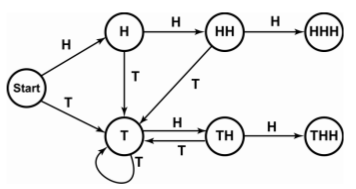
\includegraphics[width=0.6\linewidth]{RaceBetweenHHHandTHH.png}
\captionof{figure}{Markov chain for the probability of HHH or THH appearing first \cite{nickerson}}
\end{center}

To visualize the game, consider the above graph where each vertex represents the current running
for who is winning and each edge represents the probability of getting H or T. Since the probability 
of each state only depends on the previous state, we can calculate the probability $P(\tau_A < \tau_B)$
by writing a system of $n+1$ equations. 

%----------------------------------------------------------------------------------------
%	Non Transitivity
%----------------------------------------------------------------------------------------

\color{Black} % DarkSlateGray color for the rest of the content

\section{\LARGE Non Transitivity}

This game has the property that no matter what sequence A chooses, player B can choose
a $B$ such that $P(\tau_B < \tau_A) > \frac{1}{2}$. This is called non transitivity.

Guibas and Odlyzko point out that for large $n$, $a_1$ can be chosen so that
player B has odds of beating player A of $\frac{q}{q-1}$. \cite{guibas} \\

\begin{center}
%\vspace{1cm}
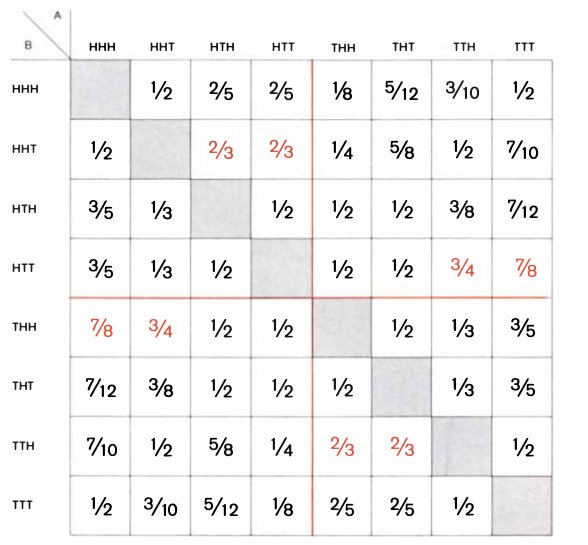
\includegraphics[width=.8\linewidth]{nonTransitivityTable.png}
\captionof{figure}{A table showing  $P(\tau_B < \tau_A)$. As an exercise, pick an A (a column), and try
to find a row in that column with a value over $\frac{1}{2}$. \cite{gardner}}
\end{center}

%----------------------------------------------------------------------------------------
%	Martingales
%----------------------------------------------------------------------------------------

\color{Black} % DarkSlateGray color for the rest of the content

\section{\LARGE Martingales}

\begin{definition}[\cite{li}]
	A martingale is a stochastic sequence $S = s_1, s_2, ...$ such that for any
	integer $k$ and for any finite expected value $E(|s_k|)$,
	$$E(s_{k+1} | s_1, ..., s_k) = s_k$$		
\end{definition}

Note that although Markov chains and martingales are both stochastic sequences, they differ
in that Markov chains is a stochastic sequence such that
the next state in the process depends only on the current state. A martingale is a
stochastic sequence such that the expected payoff in a martingale is constant. \\
In the coin flipping game, imagine at each time $t$, a gambler
is allowed to pay a wager of $w$ on the next coin flip. If they are correct, they will
win $2w$ otherwise they receive $0$. The gambler is allowed to play for however long they
want and can employ a stopping strategy for example, stop if they lose twice in a row or
bet on THH and stop. We denote the earnings of the gambler for $s$ bets starting at time
$t$ as $N_t^s$. It turns out that $N_t^s$ is a martingale and has the property that
$E(N_t^s) = 0$.
\cite{textbook}


%----------------------------------------------------------------------------------------
%	Combinatoric Method
%----------------------------------------------------------------------------------------

\color{Black} % DarkSlateGray color for the rest of the content

\section{\LARGE Combinatoric Method}


% According to Guibas and Odlyzko, the $A \oplus A$ quantity defined in Conway's algorithm
% represents the period of overlap of A with itself \cite{guibas}.

The notion of counting the period of subsequence overlaps is the basis for the combinatorial
approach for solving the penney ante problem for a generalized $q$-alphabet. We can count 
subsequences using Conway's algorithm presented in the next section.


%----------------------------------------------------------------------------------------
%	Conway's Algorithm
%----------------------------------------------------------------------------------------

\color{Black} % DarkSlateGray color for the rest of the content

\section{\LARGE Conway's Algorithm}

\begin{theorem}(Conway's Algorithm \cite{gardner})
	Given two n-tuples A and B, we find the binary representation of
	the operation $A \oplus B$ by the following algorithm:
	\begin{enumerate}
	\item loop through integers 1, 2, ..., n,
	\item At every ith iteration we look at the ith through nth digits of A and compare
	   it to the 1st through the (n-i)th digits of B.
	\item If these subsequences are equal, the ith digit in the binary representation is 1 but 0 otherwise.
	\end{enumerate}

The binary representation of $A \oplus B$
is then converted to a decimal number. Once we find $A \oplus A$, $A \oplus B$,
$B \oplus A$, and $B \oplus B$, the probability that A precedes B is
$$ \frac{A \oplus A - A \oplus B}{(B \oplus B - B \oplus A) + (A \oplus A - A \oplus B)} $$
Furthermore, 
$$E(\tau_A) = 2 (A\oplus A) $$ 

Consider $THTH \oplus THTH$ as an example.  
\begin{lstlisting}[escapechar=\%]
1010 
%\underline{THTH}%
THTH
 THTH
  THTH 
   THTH 
\end{lstlisting}

The binary number 1010 in decimal is 9 so $E(\tau_{THTH}) = 18$.

\end{theorem}

%----------------------------------------------------------------------------------------
%	Further Research
%----------------------------------------------------------------------------------------

\section{\LARGE Further Research}

This paper examines string searching for $q=2$ and general $q$ alphabet strings of length $n$.
 However, what happens when searching for a $q$ alphabet string that is biased towards certain
  letters in the alphabet? Another potential area of research is examining properties of
  nontransitive games in general, outside of this game.

%----------------------------------------------------------------------------------------
%	REFERENCES
%----------------------------------------------------------------------------------------

\nocite{*} % Print all references regardless of whether they were cited in the poster or not
\small \begin{thebibliography}{1}
	\bibitem{boyer}
		Boyer, Robert S., and J. Strother Moore. "A Fast String Searching Algorithm." Communications of the ACM 20.10 (1977): 762-72. Web.
	\bibitem{breen}
		Breen, Stephen, Waterman Michael S., and Zhang Ning. "Renewal Theory for Several Patterns." Journal of Applied Probability 22.1 (1985): 228-34. Web.
	\bibitem{gardner}
		Gardner, Martin. "Mathematical Games: On the Paradoxical Situations That Arise from Nontransitive Relations." Scientific American 10 (1974): 120-25. Print.
	\bibitem{guibas}
		Guibas, L.j, and A.m Odlyzko. "String Overlaps, Pattern Matching, and Nontransitive Games." Journal of Combinatorial Theory, Series A 30.2 (1981): 183-208. Web.  Guibas, L.j, and A.m Odlyzko. "String Overlaps, Pattern Matching, and Nontransitive Games." Journal of Combinatorial Theory, Series A 30.2 (1981): 183-208. Web.
	\bibitem{li}
		Li, Shuo-Yen Robert. "A Martingale Approach to the Study of Occurrence of Sequence Patterns in Repeated Experiments." The Annals of Probability 8.6 (1980): 1171-176. Web.
	\bibitem{nickerson}
		Nickerson, R. S. "Penney Ante: Counterintuitive Probabilities in Coin Tossing." The UMAP Journal 28.4 (2007): 503-32. JSTOR. Web. 8 Sept. 2016.
	\bibitem{textbook}
		Levin, David Asher, Y. Peres, and Elizabeth L. Wilmer. Markov Chains and Mixing times. Providence, RI: American Mathematical Society, 2009. Print.
\end{thebibliography}
			
%----------------------------------------------------------------------------------------
%	ACKNOWLEDGEMENTS
%----------------------------------------------------------------------------------------

\section*{\LARGE Acknowledgements}

\large A great BIG thank you to Curtis Greene for suggesting this idea as a thesis and
guiding me with this process.
%----------------------------------------------------------------------------------------

\end{multicols}
\end{document}
